\chapter{Tools e Tecnologie}\label{chapter:Tools-Tecnologie}

Esploriamo ora i principali strumenti e le tecnologie OSINT che possono essere utilizzate per monitorare e analizzare le attività del dark web. Questi strumenti permettono alle aziende e alle organizzazioni di individuare le proprie vulnerabilità, raccogliendo informazioni sui dati esposti e sulle potenziali minacce. L'individuazione dei possibili punti deboli, che possono favorire un attacco, è fondamentale per rafforzare le difese di sicurezza informatica e prevenire attacchi mirati. \\
Di seguito, vedremo i principali tools utilizzati per raccogliere, analizzare e proteggere le infrastrutture aziendali nel contesto della Cybersecurity.

\begin{figure}[H]
	\centering
	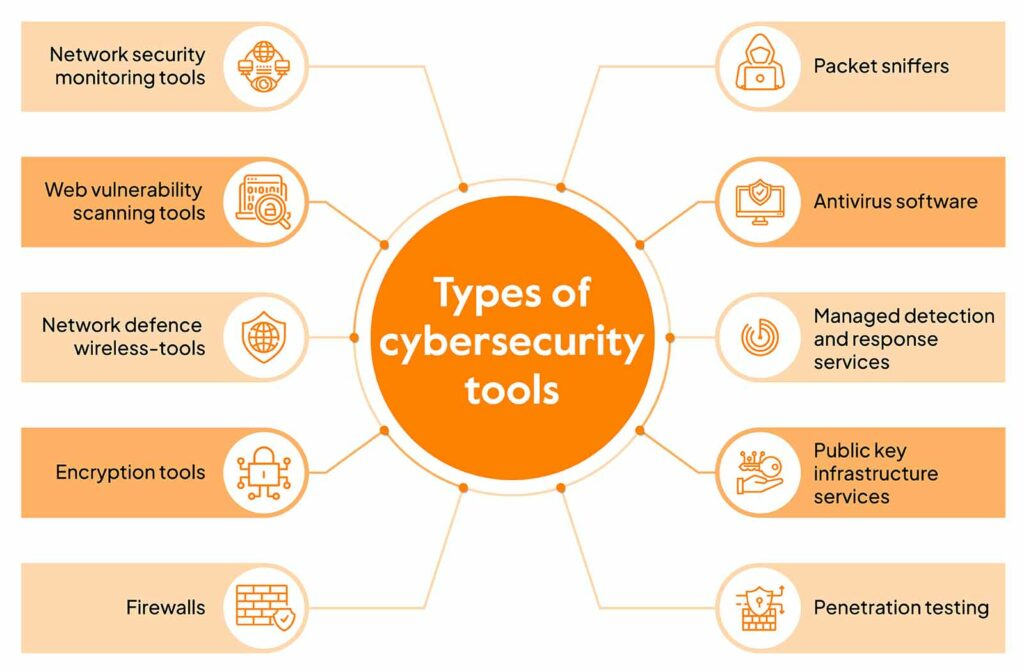
\includegraphics[width=0.9\textwidth]{Immagini/tools1.jpg}
	\caption{Tipologie di strumenti per la cybersecurity}
	\label{fig:onetools}
\end{figure}

Studieremo ora gli strumenti, analizzando le loro caratteristiche principali, funzionalità ed utilizzi. Ogni strumento offre un set unico di capacità che possono essere utilizzate per supportare le operazioni di intelligence e sicurezza. Tra questi, includiamo framework di raccolta OSINT come OSINT Framework, strumenti di data mining come Maltego, motori di ricerca per dispositivi come Shodan e Censys, piattaforme di penetration testing come Metasploit,

\section{OSINT Framework}\label{sec:cap_sec_tool1}

\textbf{OSINT Framework} è una directory completa di strumenti e risorse OSINT gratuiti disponibili online, ospitata sulla piattaforma per sviluppatori GitHub. Questo framework rappresenta un punto di partenza ideale sia per hacker che per investigatori di cybersecurity che cercano strumenti specifici per la raccolta, l'elaborazione e l'analisi di intelligence. Include una vasta gamma di dati provenienti da internet, piattaforme di social media, registri pubblici, notiziari, pubblicazioni accademiche e altri materiali open-source, offrendo un supporto strutturato per approfondire le funzionalità necessarie in un ambiente di intelligence.

\subsection{Caratteristiche ed Utilizzo}\label{subsec:es_subsec_tool1}

OSINT Framework:

\begin{enumerate}
    \item Opera entro i confini legali ed etici, poiché si basa su informazioni disponibili pubblicamente. Questo riduce i rischi associati all'accesso non autorizzato ai dati, garantendo la conformità con le leggi e le normative.
    \item Il framework OSINT consente la raccolta e l'analisi di informazioni provenienti da una vasta gamma di fonti aperte, fornendo una visione completa del panorama dell'intelligence. Questo approccio può rivelare connessioni, che potrebbero non essere evidenti con l'utilizzo di una singola fonte, portando a decisioni più accurate.
    \item Il framework OSINT permette una raccolta proattiva di intelligence, consentendo alle organizzazioni di anticipare e rispondere a potenziali minacce. Monitorando continuamente le fonti gli analisti possono identificare tendenze emergenti.
    \item La versatilità del framework OSINT lo rende applicabile a una vasta gamma di domini e soggetti.
    \item Il framework OSINT è dinamico e adattabile, consentendo l'aggiunta di nuovi strumenti, tecniche e metodologie man mano che il panorama evolve.
\end{enumerate}

\begin{figure}[ht]
	\centering
	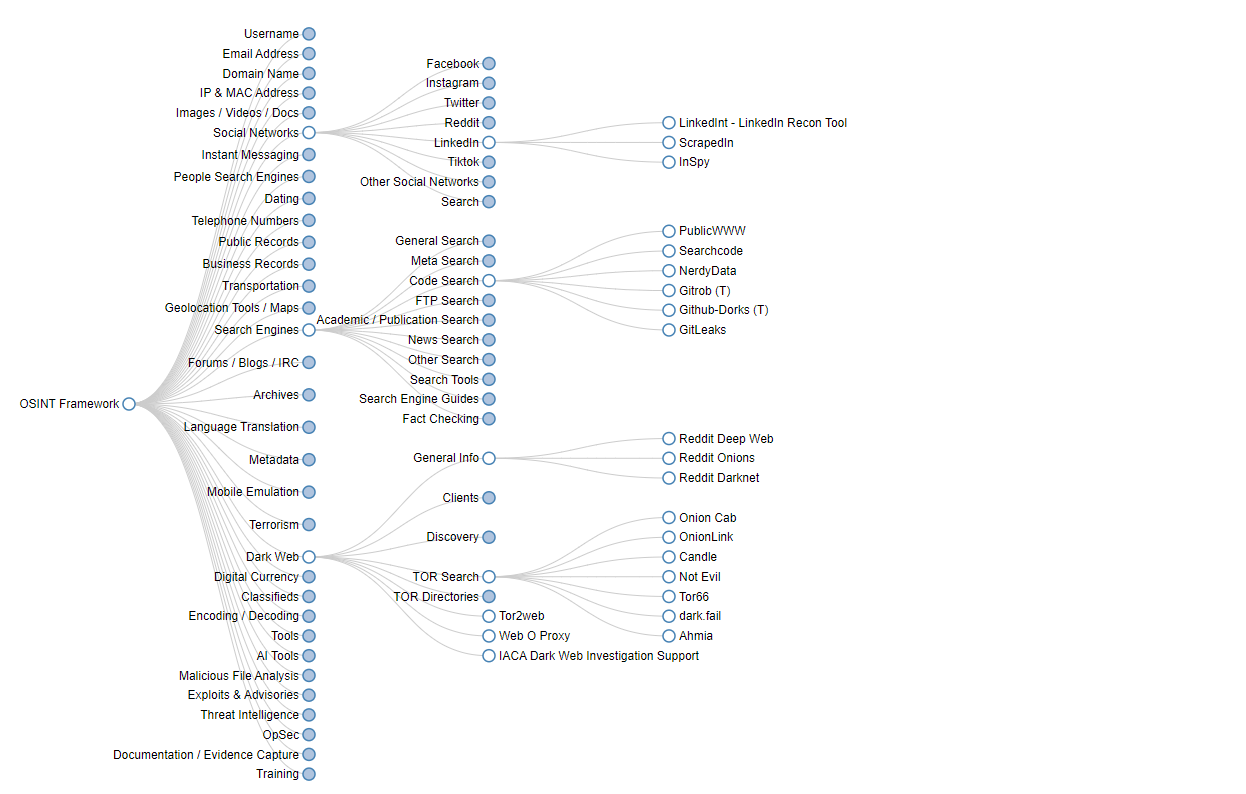
\includegraphics[width=1.2\textwidth]{Immagini/tools2.png}
	\caption{OSINT Framework}
	\label{fig:twotools}
\end{figure}


\section{Maltego}\label{sec:cap_sec_tool2}

\textbf{Maltego} è una soluzione di data mining in tempo reale e di analisi visiva disponibile per Windows, Mac e Linux. Questo strumento è progettato per identificare e visualizzare le relazioni tra varie tipologie di informazioni, come dati personali, dati aziendali, indirizzi IP, domini, e altro ancora, fornendo rappresentazioni grafiche di dati e connessioni.
Ha la capacità di profilare e tracciare le attività online degli utenti, ed è estremamente utile per gli investigatori impegnati nella sicurezza informatica, per mappare connessioni tra utenti sospetti e attività di cybercrime, individuare minacce, hacker,  e per gli analisti per identificare possibili minacce per l'organizzazione.

\subsection{Caratteristiche ed Utilizzo}\label{subsec:es_subsec_tool2}

\begin{enumerate}
    \item Esegue il data mining in tempo reale da diverse fonti online e locali, recuperando informazioni come indirizzi IP, nomi di dominio, indirizzi email, identità sui social media e numeri di telefono.
    \item Una delle caratteristiche di Maltego è la sua capacità di visualizzare relazioni complesse tra diversi tipi di dati. Utilizza grafici per mostrare le connessioni tra nodi rilevate, rendendo facile per gli analisti vedere come le informazioni sono collegate tra loro.
    \item Maltego utilizza "Transforms"\footnote{O Trasformate, sono una serie di funzioni o blocchi che permettono di estrarre e analizzare informazioni da varie fonti, essenzialmente script o moduli per trasformare i dati} per convertire una tipologia di informazione in un'altra.
    \item Gli utenti possono personalizzare le Transforms, i grafici e le visualizzazioni in base alle loro esigenze specifiche, rendendo lo strumento completamente customizzabile.
    \item È poi possibile integrare Maltego con altre piattaforme di intelligence come Shodan, Censys ecc.
\end{enumerate}

\begin{figure}[ht]
	\centering
	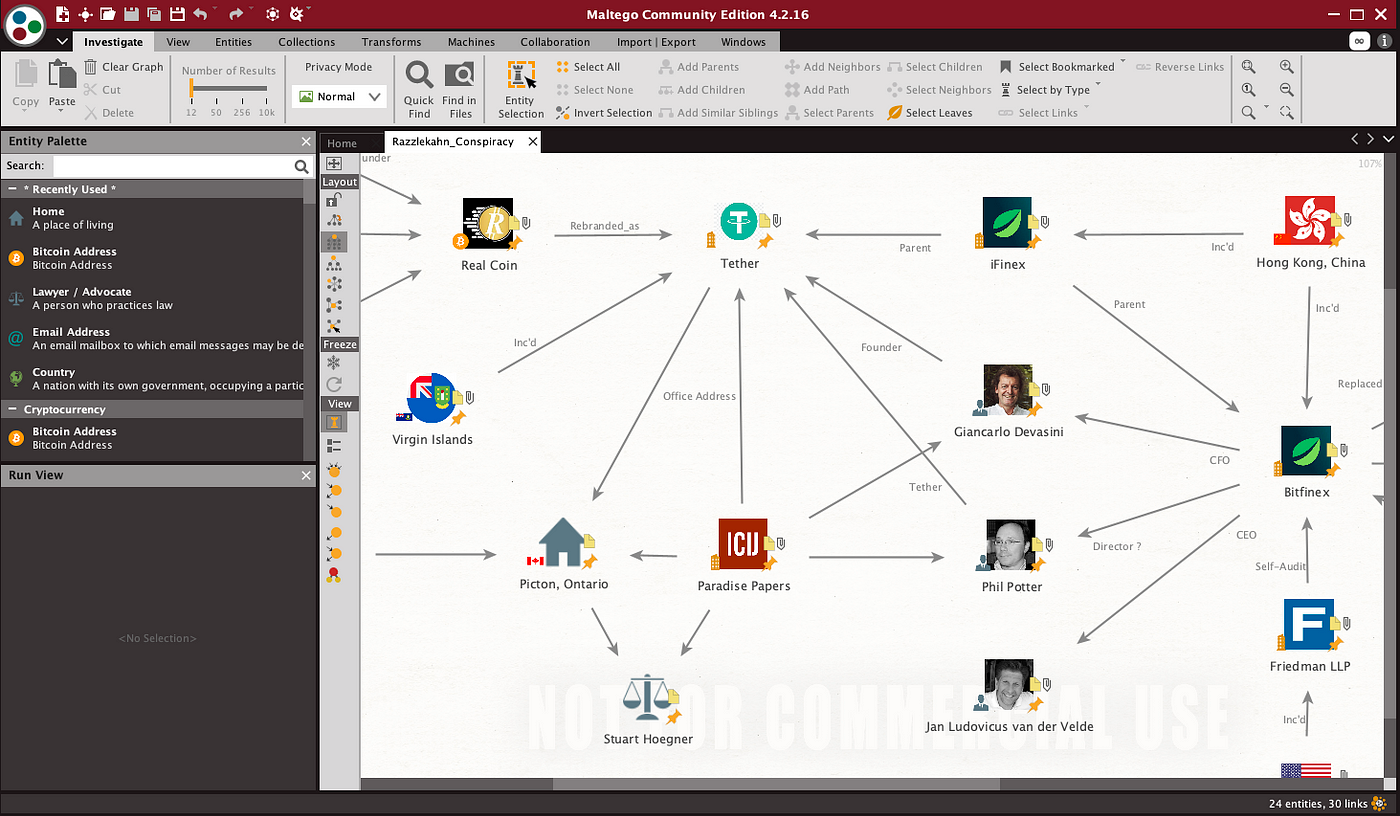
\includegraphics[width=0.95\textwidth]{Immagini/tools3.png}
	\caption{Esempio di tracciamento con Maltego}
	\label{fig:threetools}
\end{figure}

\section{SpiderFoot}\label{sec:cap_sec_tool3}

\textbf{SpiderFoot} è uno strumento di Open Source Intelligence che integra dati da una vasta gamma di fonti, inclusi il dark web, il surface web, e diverse API. È in grado di raccogliere informazioni come indirizzi e-mail, numeri di telefono, indirizzi IP, sottodomini e molto altro, offrendo un'ampia panoramica delle informazioni pubblicamente disponibili, che potrebbero rappresentare una minaccia per un'organizzazione o un individuo. SpiderFoot è uno strumento prezioso per hacker etici e professionisti della cyber security, è ideale per la scoperta automatizzata di informazioni sensibili e può essere utilizzato per scansionare il dark web alla ricerca di credenziali compromesse, dati all'interno di forum frequentati da hacker, o discussioni su potenziali vulnerabilità.

\subsection{Caratteristiche ed Utilizzo}\label{subsec:es_subsec_tool3}

\begin{enumerate}
    \item Esegue la raccolta automatizzata di informazioni da oltre 200 fonti OSINT, come DNS, registri WHOIS, motori di ricerca, piattaforme di social media, dark web e altre API pubbliche.
    \item Offre una vasta gamma di moduli che possono essere configurati per adattarsi alle esigenze specifiche dell'utente.
    \item Offre sia un'interfaccia web user-friendly sia CLI, consentendo agli utenti di eseguire scansioni e analizzare i risultati in modo flessibile.
    \item Supporta l'integrazione con strumenti di sicurezza popolari e framework di analisi come Maltego, MISP e altre piattaforme di sicurezza e produce report che possono essere esportati in diversi formati (PDF, CSV, JSON).
\end{enumerate}


\section{Shodan}\label{sec:cap_sec_tool4}

\textbf{Shodan} è un motore di ricerca online che consente di identificare server, router, webcam, e altri dispositivi esposti pubblicamente. Definita anche il "Google dei dispositivi IoT\footnote{L'Internet of Things è una rete di oggetti e dispositivi connessi e dotati di sensori e altre tecnologie che consentono loro di trasmettere e ricevere dati.}" Fornisce informazioni dettagliate sui metadati di numerosi dispositivi, sulle porte aperte e sulle vulnerabilità rilevabili. Grazie alla sua capacità di identificare dispositivi non sicuri o esposti, Shodan è uno strumento potente sia per i professionisti in ambito cybersecurity sia che per i criminali informatici. Può essere utilizzato per scoprire se i dispositivi di un'organizzazione sono visibili su Internet e se sono esposti a vulnerabilità note, un aspetto cruciale per prevenire attacchi mirati da parte di hacker che sfruttano il dark web per trovare bersagli facili.

\subsection{Caratteristiche ed Utilizzo}\label{subsec:es_subsec_tool4}

\begin{enumerate}
    \item Consente di trovare dispositivi esposti come server, router, telecamere IP, sistemi SCADA\footnote{Supervisory Control And Data Acquisition, sono sistemi con gli obbiettivi di supervisione, controllo e acquisizione dati.}, e altri dispositivi IoT. E fornisce informazioni su questi dispositivi.
    \item \'E possibile configurare avvisi per essere notificati quando nuovi dispositivi compaiono nella rete.
    \item Offre potenti filtri di ricerca che permettono di specificare dettagli come l'IP, il paese, il sistema operativo, il tipo di dispositivo e la versione del software.
    \item Fornisce dashboard intuitive e include informazioni sulle Common Vulnerabilities and Exposures (CVE) associate ai dispositivi rilevati.
\end{enumerate}

\begin{figure}[ht]
	\centering
	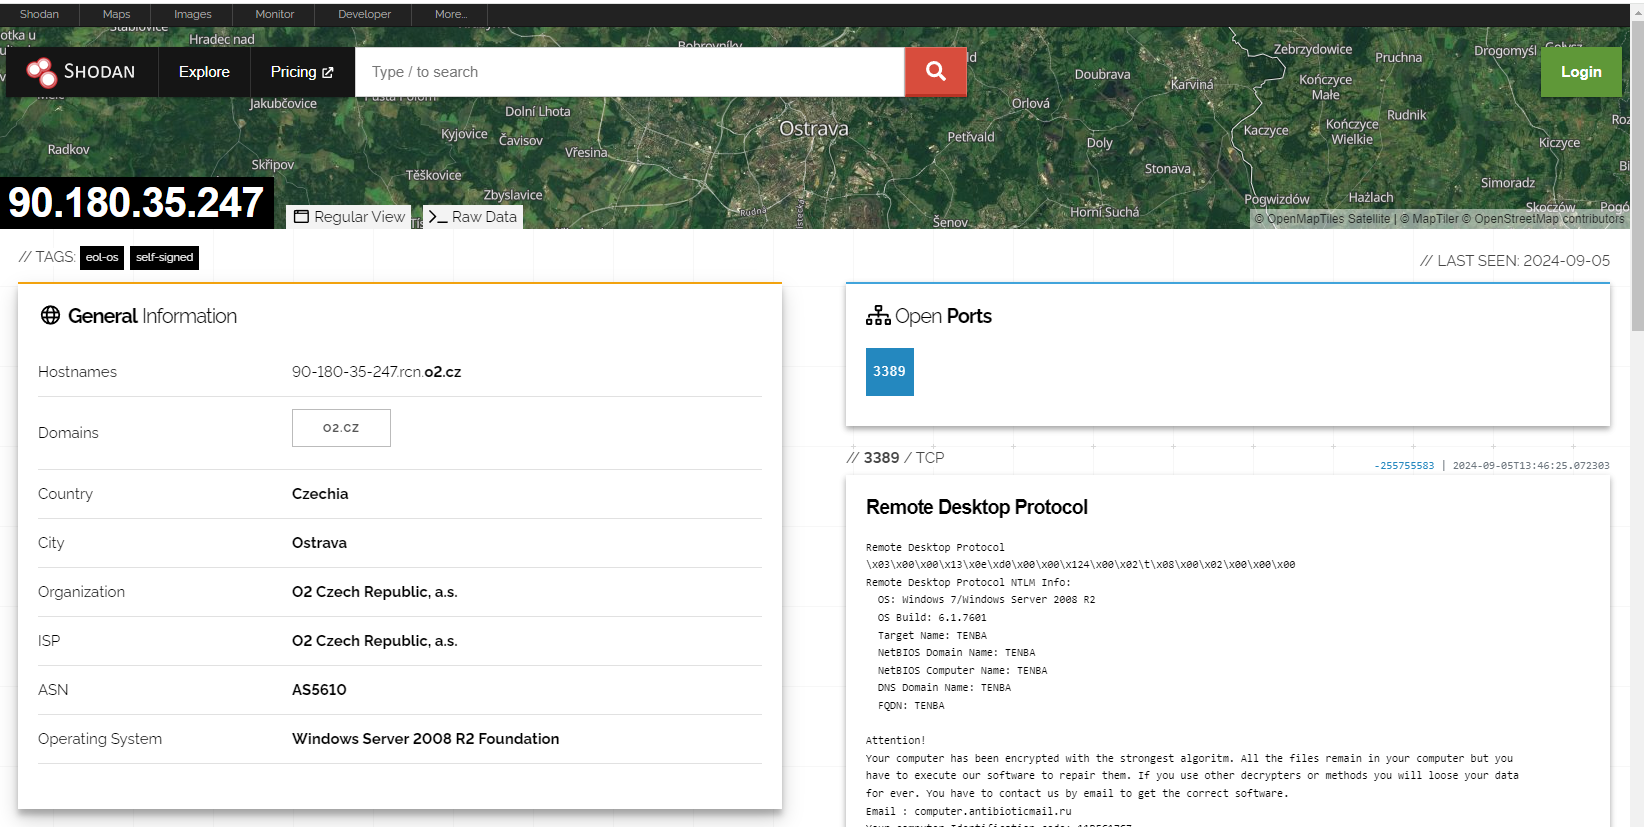
\includegraphics[width=1\textwidth]{Immagini/tools4.png}
	\caption{Server con Remote Desktop Protocol esposto}
	\label{fig:fourtools}
\end{figure}


\section{Have I Been Pwned (HIBP):}\label{sec:cap_sec_tool5}

\textbf{Have I Been Pwned} è un servizio disponibile sul clear web che consente di verificare se le credenziali aziendali o personali sono state compromesse in un data breach. Offre un database consultabile dove gli utenti possono controllare se i loro indirizzi email o le loro password sono presenti in data breach noti.
È uno strumento essenziale per le organizzazioni, poiché permette di monitorare regolarmente se le credenziali dei dipendenti sono state esposte in violazioni di dati. In caso di compromissione, consente di reagire rapidamente aggiornando le password e implementando misure di sicurezza aggiuntive, come l'autenticazione a più fattori, per mitigare i rischi di ulteriori attacchi.

\begin{figure}[ht]
	\centering
	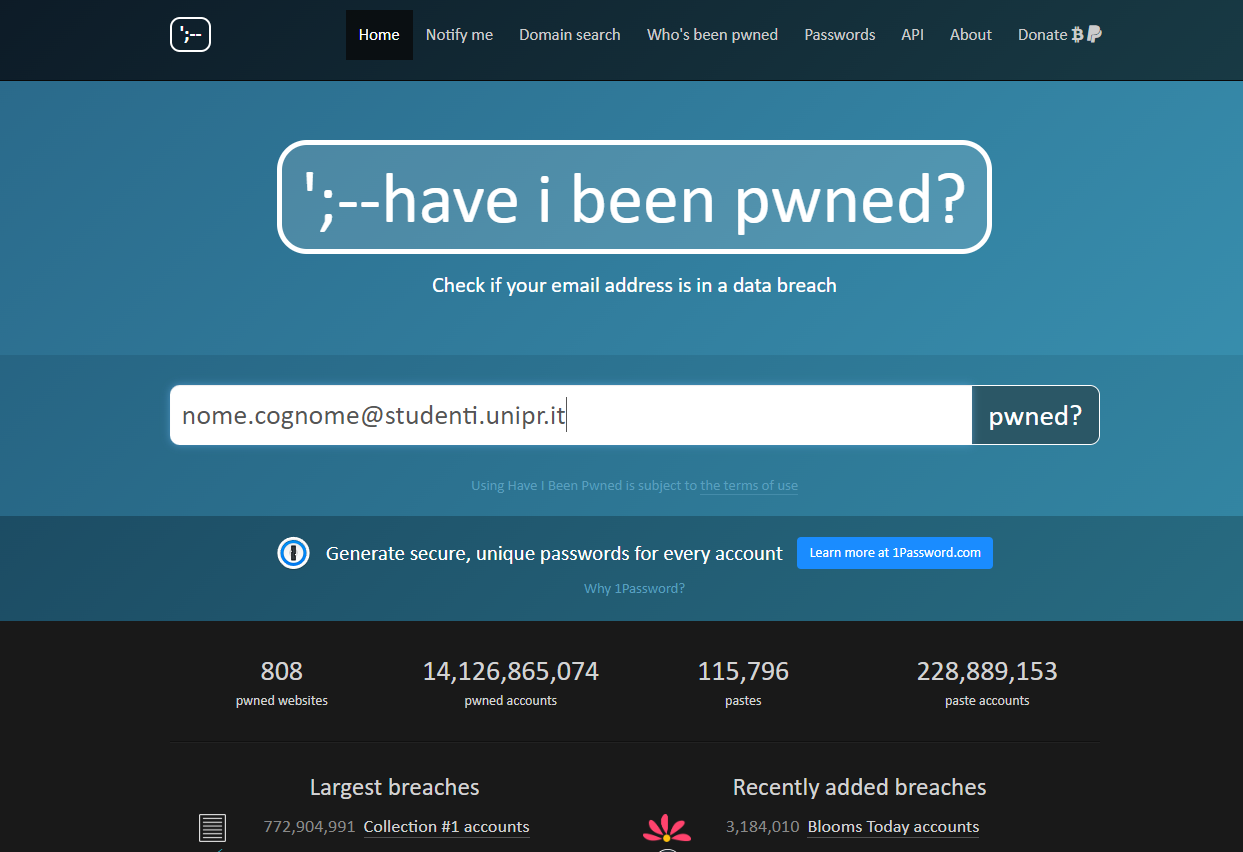
\includegraphics[width=0.9\textwidth]{Immagini/tools5.png}
	\caption{Textbox di HIBP per la verifica di credenziali}
	\label{fig:fivetools}
\end{figure}

\subsection{Caratteristiche ed Utilizzo}\label{subsec:es_subsec_tool5}

\begin{enumerate}
    \item Il database mantiene un vasto elenco di violazioni e al momento include miliardi di record provenienti da centinaia di data breach.
    \item Gli utenti possono cercare i propri indirizzi email per vedere se sono stati compromessi. E le aziende possono verificare se i domini aziendali sono presenti nei data breach per monitorare se sono presenti le credenziali dei loro dipendenti.
    \item Consente agli utenti di iscriversi al sito per ricevere un avviso in caso di nuove violazioni di dati che coinvolgono le loro credenziali.
    \item Permette di verificare se una password è stata esposta in una violazione di dati e offre un'API per dare la possibilità alle aziende di integrare questi controlli nei loro sistemi.\\
\end{enumerate}

\section{Altri strumenti utili:}\label{sec:cap_sec_tool6}

\textbf{Burp Suite:}\\
Burp Suite è uno strumento di test di sicurezza delle applicazioni web utilizzato per identificare e analizzare vulnerabilità in siti web e applicazioni online. Questo software fornisce un set completo di strumenti integrati che consentono di effettuare il crawling, lo scanning, l'analisi e la manipolazione del traffico HTTP/S. È ampiamente utilizzato da penetration tester e professionisti della sicurezza per eseguire test di sicurezza manuali e automatizzati, individuando problemi come sql injection, cross-site scripting (XSS), e altre vulnerabilità comuni. Grazie alla sua interfaccia user-friendly e alla possibilità di aggiungere estensioni, Burp Suite è considerato uno dei tool più versatili per la sicurezza delle applicazioni web.\\


\textbf{Metasploit:}\\
Metasploit è una piattaforma avanzata per il penetration testing che consente di identificare, verificare e sfruttare le vulnerabilità di sicurezza presenti in reti, sistemi, e applicazioni. Utilizzato da cybersecurity analyst, ricercatori e anche da hacker, Metasploit offre una vasta libreria di exploit, payload, e moduli per testare la sicurezza di un'infrastruttura IT. La piattaforma supporta sia attacchi manuali che automatizzati, permettendo di simulare scenari di attacco reali per valutare l'efficacia delle difese di un'organizzazione. Oltre all'identificazione delle vulnerabilità, Metasploit può essere utilizzato per test di sicurezza approfonditi, auditing, e per il miglioramento delle strategie di mitigazione dei rischi, rendendolo uno strumento versatile e indispensabile nel campo della sicurezza informatica.\\


\textbf{Recon-ng:}\\
\'E uno strumento, open-source scritto in Python, per la ricognizione e raccolta dati, progettato per automatizzare il processo di OSINT durante le attività di penetration testing e cybersecurity. È simile a Metasploit per la sua struttura modulare, ma è specificamente focalizzato sulle fasi iniziali di un attacco, in cui gli eventuali hacker cercano di raccogliere il maggior numero informazioni su un bersaglio (come domini, indirizzi IP, persone, aziende, ecc.) da fonti pubblicamente disponibili.
è altamente modulare, consentendo agli utenti di aggiungere, rimuovere e aggiornare facilmente i moduli, presenta un interfaccia a CLI\footnote{Riga di Comando} simile a quella di Metasploit, con la possibilità di eseguire comandi come add, remove, run e show. Offre poi la possibilità di generare report dettagliati in vari formati, come HTML, JSON, o CSV. Raccoglie i dati in database che poi è possibile consultare attraverso delle query.\\


\textbf{Ahmia:}\\
Definito come il motore di ricerca del dark web, è uno degli strumenti più conosciuti ed utilizzati per navigare e ricercare contenuti sul dark web in modo sicuro e organizzato. \'E uno dei pochi strumenti progettati appositamente per permette la ricerca di siti .onion all'interno della rete TOR. A differenza di altri motori di ricerca Ahmia adotta criteri di indicizzazione rigorosi. Filtra i risultati per evitare la visualizzazione di contenuti illegali o dannosi, o quelli legati a malware e attività criminali.
\'E accessibile sia dal clear web che dalla rete Tor, è un progetto open source\footnote{Il suo codice è aperto e disponibile per la revisione da parte della community} (il che garantisce un elevato livello di trasparenza riguardo alle sue operazioni), e facilita l'identificazione di tendenze emergenti o threats grazie alla sua capacità di indicizzare e filtrare il dark web.
Ahmia non traccia gli utenti e protegge la loro privacy, mantenendo una blacklist di siti che violano i suoi termini di servizio.\\


\textbf{Censys:}\\
Censys è una piattaforma di ricerca e analisi che, simile a Shodan, scansiona e fornisce informazioni dettagliate sugli asset connessi a Internet, come server, dispositivi IoT e servizi web. Tuttavia, Censys si distingue per le sue capacità di analisi più approfondite e per la sua interfaccia avanzata, che consente agli utenti di ottenere una visione più completa della superficie di attacco di un'organizzazione. La piattaforma offre anche funzionalità di monitoraggio continuo e avvisi personalizzati sulle esposizioni dei dati, permettendo di individuare rapidamente eventuali vulnerabilità o configurazioni errate. Per un'azienda, l'utilizzo di Censys è fondamentale per monitorare gli asset esposti su Internet e mitigare i rischi di accessi non autorizzati, riducendo così la probabilità di essere bersaglio di attacchi.\\


\textbf{Nmap:}\\
\'E uno strumento open-source utilizzato per la scansione e l'analisi di reti, disponibile per Windows, Linux e macOS. È uno dei tool più popolari e potenti nel campo della sicurezza informatica e del penetration testing, ed è ampiamente utilizzato da amministratori di rete, analisti di sicurezza, e hacker per la raccolta di informazioni su reti, sistemi e dispositivi.
Nmap è famoso per la sua capacità di eseguire scansioni sulle porte di un host o su una rete, identificando quali porte sono aperte e quali chiuse o filtrate. Questo permette di determinare quali servizi stanno girando su una macchina e di conseguenza se ci sono potenziali vulnerabilità sfruttabili. Può identificare il sistema operativo di un dispositivo, può anche identificare i servizi che stanno girando su quelle porte (ad esempio, un server web su HTTP o un server FTP\footnote{File Transfer Protocol è un protocollo di comunicazione usato per il trasferimento di file da un server a un client}.
Il Nmap Scripting Engine (NSE) è una delle sue funzionalità più importanti, e consente di eseguire script che possono automatizzare un'ampia gamma di attività di rete, dal rilevamento di vulnerabilità comuni all'esecuzione di attacchi di brute-force, è progettata per essere efficiente anche operando su una grande mole di dati.\\


\textbf{Dark Web Monitoring Tools (ad esempio, DarkOwl, Recorded Future):}\\
Questi sono strumenti avanzati progettati per aiutare le organizzazioni a monitorare il dark web alla ricerca di informazioni compromesse riguardo l'azienda. Questi strumenti possono identificare dati sensibili come credenziali violate, documenti riservati, o discussioni su possibili attacchi futuri che potrebbero rappresentare una minaccia per la sicurezza aziendale.
Offrono un monitoraggio continuo delle menzioni di un'organizzazione sul dark web, consentendo di individuare rapidamente eventuali fughe di dati o attività sospette pianificate contro l'azienda. Questa capacità di rilevamento tempestivo è cruciale per prevenire danni, permettendo alle organizzazioni di adottare misure di risposta rapida e rafforzare le loro difese di sicurezza.\\


\textbf{DarkOwl:}\\
\'E una piattaforma di intelligence specializzata nella raccolta, analisi e monitoraggio di dati dal dark web, dal deep web e altre fonti non indicizzate dai motori di ricerca tradizionali. Viene utilizzato da diversi attori, DarkOwl aiuta le organizzazioni a identificare minacce, informazioni compromesse e attività malevole che potrebbero rappresentare un rischio per la sicurezza.
utilizza tecnologie avanzate per la raccolta automatizzata di dati dal dark web, e si focalizza su "Darknet Intelligence" (DarkInt), ossia l'intelligence derivata da contenuti e attività nascoste nel dark web. Infine fornisce una dashboard intuitiva per l'analisi e la visualizzazione dei dati.\\


\textbf{Recorded Future:}\\
\'E una piattaforma di Threat Intelligence basata sull'intelligenza artificiale e sull'analisi predittiva, progettata per aiutare le organizzazioni a identificare e mitigare le minacce alla sicurezza informatica in modo proattivo, unisce dati raccolti da milioni di fonti, allo scopo di fornire informazioni dettagliate e contestuali sulle minacce informatiche. Utilizza algoritmi di machine learning e NLP\footnote{Natural Language Processing} per analizzare automaticamente grandi volumi di dati. Una delle caratteristiche distintive è la sua capacità di fornire informazioni per ogni minaccia identificata (chi è coinvolto, la cronologia degli eventi, le motivazioni degli attaccanti, e la potenziale gravità).\\


\textbf{Threat Intelligence Platforms (TIPs):}\\
Le piattaforme come MISP (Malware Information Sharing Platform) sono strumenti utilizzati per raccogliere, organizzare e condividere informazioni riguardanti minacce note ed emergenti. Questi strumenti permettono di centralizzare le informazioni per facilitare l'analisi e la risposta alle stesse.
Le TIPs aiutano le organizzazioni a gestire i dati OSINT raccolti sulle minacce conosciute, supportando la definizione di contromisure efficaci. Permettono di monitorare proattivamente le minacce, consente di rafforzare la sicurezza complessiva, e rispondere a potenziali rischi in modo tempestivo.\\


\textbf{Social Media Intelligence Tools:}\\
Questi strumenti (ad esempio, Social Searcher, Mentionlytics) consentono di monitorare le menzioni dell'azienda e dei suoi dipendenti sui social media, piattaforme spesso sfruttate dagli hacker per raccogliere informazioni e preparare attacchi mirati.
Utilizzando questi strumenti, le organizzazioni possono individuare potenziali campagne di phishing, disinformazione, o attacchi di social engineering pianificati. Questo monitoraggio aiuta a prevenire incidenti e a mantenere alta la reputazione dell'azienda, permettendo di reagire tempestivamente a minacce emergenti.\\


\textbf{VPN e TOR:}\\
L'utilizzo di VPN e del browser TOR è cruciale per garantire sicurezza e anonimato durante le attività di monitoraggio del dark web. Questi strumenti criptano il traffico internet e nascondono l'indirizzo IP dell'utente, rendendo difficile la tracciabilità.
Minimizzare il rischio di rilevamento da parte di hacker è fondamentale per chi conduce operazioni di intelligence sul dark web. Utilizzando VPN e Tor, gli investigatori possono navigare in modo sicuro e anonimo, riducendo al minimo le possibilità di essere identificati o monitorati durante le indagini su attività sospette o minacce emergenti.\\


\textbf{Elastic Stack (ELK):}\\
Elastic Stack, comunemente noto come ELK Stack, è una suite di strumenti open source composta da Elasticsearch, Logstash, e Kibana, progettata per la ricerca, l'analisi e la visualizzazione di grandi volumi di dati in tempo reale. \textbf{Elasticsearch} è un motore di ricerca e analisi distribuito, \textbf{Logstash} è uno strumento per l'ingestione, l'elaborazione e l'arricchimento dei dati, mentre \textbf{Kibana} offre potenti funzionalità di visualizzazione dei dati e creazione di dashboard.
Elastic Stack è ampiamente utilizzato sui log provenienti da diversi sistemi all'interno di un'organizzazione. Nel contesto della sicurezza informatica, può essere impiegato per monitorare i segnali di compromissione (Indicators of Compromise, IoC), identificando potenziali minacce associate al dark web. L'ELK Stack consente di centralizzare i log di sicurezza, analizzare anomalie nel traffico di rete, tracciare attività sospette e generare avvisi in tempo reale, migliorando così la capacità dell'organizzazione di rilevare e rispondere rapidamente agli incidenti di sicurezza.\\


\textbf{Splunk:}\\
Software che permette di cercare, monitorare e analizzare grandi volumi di dati generati da macchine in tempo reale. Viene utilizzato principalmente per l'analisi di log e per la gestione delle operazioni IT e per il monitoraggio delle applicazioni.
Splunk può raccogliere dati da diverse fonti, come server, reti, applicazioni, sensori IoT, e sistemi operativi. Utilizza un proprio linguaggio di ricerca chiamato SPL (Search Processing Language) e offre strumenti per la visualizzazione dei dati attraverso grafici, dashboard, e report, che possono essere personalizzati per visualizzare l’andamento dei dati nel tempo.\\


\textbf{Nessus:}\\
Strumento per la scansione di vulnerabilità, utilizzato per identificare potenziali punti deboli, problemi di configurazione e falle di sicurezza in reti, server, applicazioni e altri dispositivi informatici.
Nessus è in grado di eseguire scansioni su una vasta gamma di dispositivi e sistemi operativi, rilevando, vulnerabilità note, porte aperte, configurazioni errate, software obsoleto. Utilizza un vasto database di vulnerabilità aggiornato regolarmente. \'E possibile programmare scansioni automatiche a intervalli regolari, con i quali generare report dettagliati e creare report personalizzati.\\

\newpage
\textbf{MISP (Malware Information Sharing Platform):}\\
Piattaforma open source progettate per facilitare la condivisione, l'aggregazione e l'analisi di informazioni relative alle minacce. Utilizzata da organizzazioni, governi e comunità si cybersecurity in tutto il mondo. \'E uno strumento utile per migliorare la consapevolezza situazionale delle minacce e la loro risposta.
Consente la condivisione strutturata di informazioni su malware, indicatori di compromissione (IoC), tattiche, tecniche e procedure (TTP) degli attaccanti, vulnerabilità e altre informazioni utili.
MISP è progettato per supportare la collaborazione tra diverse entità, come team di sicurezza interni, CERT\footnote{Computer Emergency Response Teams}, CSIRT\footnote{Computer Security Incident Response Teams}, e altre entità di difesa dell'organizzazione.
\'E dotato di robusti controlli di accesso e può essere integrato con altre piattaforme di sicurezza informatica attraverso API e script personalizzati.\\


Questi sono solo alcuni degli strumenti che andremo ad analizzare e ad utilizzare.

